\documentclass[11pt]{article}

% ---------------------------------------------------------------------------
% Packages
% ---------------------------------------------------------------------------
\usepackage[margin=1in]{geometry}
\usepackage[T1]{fontenc}
\usepackage{graphicx}
\usepackage{longtable}
\usepackage{booktabs}
\usepackage{array}
\usepackage{enumitem}
\usepackage{xcolor}
\usepackage{hyperref}
\usepackage{tikz}
\usepackage{float}
\usepackage{fancyhdr}
\usepackage{titlesec}
\usepackage{tcolorbox}
\tcbuselibrary{breakable}
\usepackage{tabularx}
\usepackage{multirow}
\usepackage{caption}
\usepackage{listings}
\usepackage{makecell}
\usepackage{amssymb}
\usepackage{pifont}

\usetikzlibrary{shapes.geometric, arrows.meta, positioning, fit, backgrounds, calc, decorations.pathreplacing, shapes.multipart, matrix, shadows}

% ---------------------------------------------------------------------------
% Color Definitions
% ---------------------------------------------------------------------------
\definecolor{sectionblue}{RGB}{31,78,121}
\definecolor{modulecolor}{RGB}{70,130,180}
\definecolor{cnccolor}{RGB}{60,179,113}
\definecolor{alloccolor}{RGB}{255,165,0}
\definecolor{flowcolor}{RGB}{100,100,100}
\definecolor{lightgray}{RGB}{245,245,245}
\definecolor{warningred}{RGB}{220,53,69}
\definecolor{successgreen}{RGB}{40,167,69}
\definecolor{infoblue}{RGB}{23,162,184}
\definecolor{decisioncolor}{RGB}{186,85,211}
\definecolor{externalcolor}{RGB}{255,193,7}
\definecolor{datacolor}{RGB}{144,238,144}

\hypersetup{
  colorlinks=true,
  linkcolor=sectionblue,
  urlcolor=sectionblue,
  citecolor=sectionblue
}

% ---------------------------------------------------------------------------
% Header and Footer
% ---------------------------------------------------------------------------
\pagestyle{fancy}
\setlength{\headheight}{14pt}
\addtolength{\topmargin}{-2pt}
\fancyhf{}
\fancyhead[L]{\leftmark}
\fancyhead[R]{Architecture Documentation}
\fancyfoot[C]{\thepage}
\renewcommand{\headrulewidth}{0.4pt}
\renewcommand{\footrulewidth}{0.4pt}

% ---------------------------------------------------------------------------
% Section Formatting
% ---------------------------------------------------------------------------
\titleformat{\section}
  {\normalfont\Large\bfseries\color{sectionblue}}{\thesection}{1em}{}
\titleformat{\subsection}
  {\normalfont\large\bfseries\color{sectionblue!80}}{\thesubsection}{1em}{}
\titleformat{\subsubsection}
  {\normalfont\normalsize\bfseries\color{sectionblue!60}}{\thesubsubsection}{1em}{}

% ---------------------------------------------------------------------------
% Custom Box Environments
% ---------------------------------------------------------------------------
\newtcolorbox{keypoint}{
    colback=blue!5,
    colframe=sectionblue,
    title=Key Point,
    fonttitle=\bfseries
}

\newtcolorbox{warning}{
    colback=red!5,
    colframe=warningred,
    title=Warning,
    fonttitle=\bfseries
}

\newtcolorbox{bestpractice}{
    colback=green!5,
    colframe=successgreen,
    title=Best Practice,
    fonttitle=\bfseries
}

\newtcolorbox{example}{
    colback=lightgray,
    colframe=flowcolor,
    title=Example,
    fonttitle=\bfseries
}

\newtcolorbox{definition}{
    colback=infoblue!10,
    colframe=infoblue,
    title=Definition,
    fonttitle=\bfseries
}

\newtcolorbox{template}{
    colback=white,
    colframe=flowcolor,
    title=Template,
    fonttitle=\bfseries
}

\newtcolorbox{viewbox}[1][]{
    colback=modulecolor!5,
    colframe=modulecolor,
    title=#1,
    fonttitle=\bfseries,
    breakable
}

\newtcolorbox{decisionbox}[1][]{
    colback=decisioncolor!10,
    colframe=decisioncolor,
    title=#1,
    fonttitle=\bfseries
}

% ---------------------------------------------------------------------------
% Code Listing Style
% ---------------------------------------------------------------------------
\lstset{
    basicstyle=\ttfamily\small,
    breaklines=true,
    frame=single,
    backgroundcolor=\color{lightgray},
    keywordstyle=\color{sectionblue},
    commentstyle=\color{successgreen},
    stringstyle=\color{alloccolor},
    showstringspaces=false
}

% ---------------------------------------------------------------------------
% Custom Column Types
% ---------------------------------------------------------------------------
\newcolumntype{L}[1]{>{\raggedright\arraybackslash}p{#1}}
\newcolumntype{C}[1]{>{\centering\arraybackslash}p{#1}}
\newcolumntype{R}[1]{>{\raggedleft\arraybackslash}p{#1}}

% ---------------------------------------------------------------------------
% Simple styling helpers
% ---------------------------------------------------------------------------
\setlist[itemize]{topsep=3pt,itemsep=2pt,parsep=0pt}
\setlist[enumerate]{topsep=3pt,itemsep=2pt,parsep=0pt}

% Status commands
\newcommand{\statusdraft}{\textcolor{infoblue}{\textbf{[DRAFT]}}}
\newcommand{\statusreview}{\textcolor{alloccolor}{\textbf{[REVIEW]}}}
\newcommand{\statusapproved}{\textcolor{successgreen}{\textbf{[APPROVED]}}}
\newcommand{\statusdeprecated}{\textcolor{flowcolor}{\textbf{[DEPRECATED]}}}

% ---------------------------------------------------------------------------
% Project-specific metadata
% ---------------------------------------------------------------------------
\newcommand{\ProjectName}{E-Commerce Platform Modernization}
\newcommand{\SystemName}{OrderFlow Commerce Platform}
\newcommand{\docid}{ARCH-DOC-001}
\newcommand{\docversion}{2.1.0}
\newcommand{\docstatus}{Approved}
\newcommand{\docowner}{Architecture Team}
\newcommand{\docapprover}{Chief Architect}

% ---------------------------------------------------------------------------
% Title
% ---------------------------------------------------------------------------
\title{%
    \vspace{-1cm}
    \textbf{\Huge Software Architecture Documentation}\\[12pt]
    \Large Comprehensive Template and Guide\\[8pt]
    \large Views and Beyond Approach for \SystemName\\[6pt]
    \normalsize Based on SEI/CMU Documentation Standards
}
\author{%
    \ProjectName\\[4pt]
    \small Architecture Documentation Series
}
\date{\today}

\begin{document}
\maketitle
\thispagestyle{empty}

\vspace{0.5cm}

\begin{abstract}
\noindent
This document provides a comprehensive architecture documentation template following the Views and Beyond approach developed by the Software Engineering Institute at Carnegie Mellon University. The template establishes a systematic framework for documenting software architectures through multiple architectural views, each addressing specific stakeholder concerns. This guide serves dual purposes: as a reference template for creating architecture documentation and as a filled-in example demonstrating best practices for a modern e-commerce platform. The document covers the complete documentation structure including view templates, element catalogs, rationale documentation, requirements traceability, and governance processes essential for maintaining architecture documentation throughout the system lifecycle.
\end{abstract}

\vfill

\begin{center}
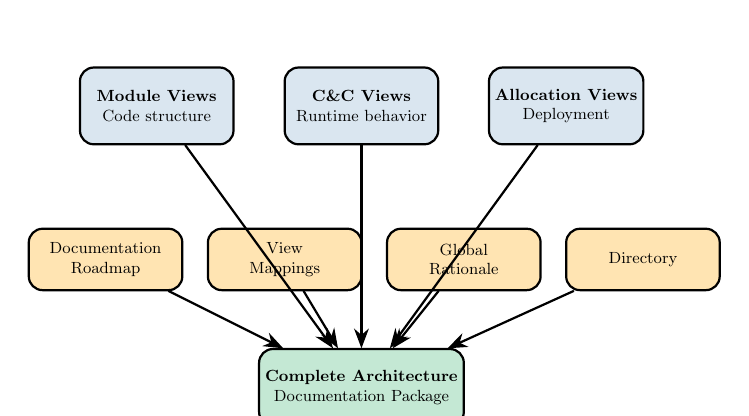
\begin{tikzpicture}[
    scale=0.65,
    transform shape,
    view/.style={draw, thick, fill=modulecolor!20, minimum width=3cm, minimum height=1.5cm, rounded corners=5pt, font=\small, align=center},
    beyond/.style={draw, thick, fill=alloccolor!30, minimum width=3cm, minimum height=1.2cm, rounded corners=5pt, font=\small, align=center},
    arrow/.style={-{Stealth[length=2.5mm]}, thick}
]
    % Views
    \node[view] (module) at (-4,2) {\textbf{Module Views}\\Code structure};
    \node[view] (cnc) at (0,2) {\textbf{C\&C Views}\\Runtime behavior};
    \node[view] (alloc) at (4,2) {\textbf{Allocation Views}\\Deployment};
    
    % Beyond
    \node[beyond] (roadmap) at (-5,-1) {Documentation\\Roadmap};
    \node[beyond] (mapping) at (-1.5,-1) {View\\Mappings};
    \node[beyond] (rationale) at (2,-1) {Global\\Rationale};
    \node[beyond] (directory) at (5.5,-1) {Directory};
    
    % Central system
    \node[draw, thick, fill=cnccolor!30, minimum width=4cm, minimum height=1.5cm, rounded corners=5pt, align=center, font=\small] (system) at (0,-3.5) {\textbf{Complete Architecture}\\Documentation Package};
    
    % Connections
    \draw[arrow] (module) -- (system);
    \draw[arrow] (cnc) -- (system);
    \draw[arrow] (alloc) -- (system);
    \draw[arrow] (roadmap) -- (system);
    \draw[arrow] (mapping) -- (system);
    \draw[arrow] (rationale) -- (system);
    \draw[arrow] (directory) -- (system);
\end{tikzpicture}
\end{center}

\newpage
\tableofcontents
\newpage

% ======================================================================
\section*{Document Control Information}
\addcontentsline{toc}{section}{Document Control Information}
% ======================================================================

\begin{table}[H]
\centering
\begin{tabular}{@{}L{4cm} L{9cm}@{}}
\toprule
\textbf{Attribute} & \textbf{Value} \\
\midrule
Document ID & \docid \\
Title & Architecture Description for \SystemName \\
Project & \ProjectName \\
Version & \docversion \\
Status & \docstatus~\statusapproved \\
Author / Owner & \docowner \\
Approver & \docapprover \\
Creation Date & 2023-06-15 \\
Last Updated & \today \\
Repository & \texttt{github.com/company/orderflow-architecture} \\
Branch/Tag & \texttt{main} / \texttt{v2.1.0} \\
Classification & Internal -- Confidential \\
Review Cycle & Quarterly \\
\bottomrule
\end{tabular}
\end{table}

\vspace{1em}

\subsection*{Change History}

\begin{longtable}{@{}L{1.2cm} L{2cm} L{2.5cm} L{7cm}@{}}
\toprule
\textbf{Version} & \textbf{Date} & \textbf{Author} & \textbf{Summary of Changes} \\
\midrule
\endfirsthead
\toprule
\textbf{Version} & \textbf{Date} & \textbf{Author} & \textbf{Summary of Changes} \\
\midrule
\endhead
\bottomrule
\endlastfoot
1.0.0 & 2023-06-15 & J. Smith & Initial architecture documentation release \\
1.1.0 & 2023-09-20 & A. Jones & Added Payment Service decomposition; updated C\&C view \\
1.2.0 & 2023-12-10 & J. Smith & Added Kubernetes deployment view; security patterns \\
2.0.0 & 2024-03-15 & Architecture Team & Major revision: microservices decomposition; event-driven patterns \\
2.1.0 & 2024-06-01 & B. Wilson & Added GraphQL gateway; updated requirements traceability \\
\end{longtable}

\vspace{1em}

\subsection*{Change Request and Review Process}

Architecture documentation changes follow a structured governance process to ensure quality and stakeholder alignment.

\begin{enumerate}
    \item \textbf{Change Request:} Submit via GitHub Issue using the ``Architecture Change'' template. Include rationale, affected views, and stakeholder impact assessment.
    
    \item \textbf{Triage:} Architecture Team reviews within 2 business days, assigns priority (Critical/High/Medium/Low), and identifies reviewers.
    
    \item \textbf{Development:} Author creates branch (\texttt{arch/description-of-change}), updates documentation, and ensures all cross-references remain valid.
    
    \item \textbf{Review:} Pull request requires approval from:
    \begin{itemize}[nosep]
        \item At least one Architecture Team member
        \item Affected subsystem technical lead
        \item Chief Architect for structural changes
    \end{itemize}
    
    \item \textbf{Release:} Merged changes trigger documentation build. Major versions announced via architecture-announce mailing list.
\end{enumerate}

\begin{keypoint}
All architecture documentation changes must be traceable to either a requirements change, an Architecture Decision Record (ADR), or a documented technical debt item.
\end{keypoint}

\newpage

% ======================================================================
\section{Documentation Roadmap}
% ======================================================================

The Documentation Roadmap provides readers with an orientation to the architecture documentation, explaining its purpose, organization, and how different stakeholders should navigate it.

\subsection{Scope and Summary}

\begin{definition}
\textbf{Architecture Documentation} captures the fundamental organization of a system embodied in its components, their relationships to each other and to the environment, and the principles guiding its design and evolution (IEEE 1471/ISO 42010).
\end{definition}

\begin{itemize}
  \item \textbf{Purpose:} This document describes the software architecture of \SystemName, a modern e-commerce platform supporting B2C and B2B transactions. It serves as the authoritative reference for architectural decisions, component responsibilities, and system structure to enable effective communication among stakeholders, guide implementation, support analysis, and facilitate evolution.
  
  \item \textbf{Scope:} The documentation covers:
  \begin{itemize}[nosep]
      \item Core platform services (Order, Inventory, Payment, User, Catalog, Search)
      \item Supporting infrastructure (API Gateway, Event Bus, Observability)
      \item External integration points (Payment providers, Shipping carriers, ERP systems)
      \item Deployment architecture (Kubernetes clusters, database tier, CDN)
  \end{itemize}
  
  \item \textbf{Out of Scope:}
  \begin{itemize}[nosep]
      \item Detailed design within individual services (covered in service-level design docs)
      \item Test strategies and plans (covered in QA documentation)
      \item Operational runbooks (covered in SRE documentation)
      \item Third-party system internals
  \end{itemize}
  
  \item \textbf{Related Artifacts:}
  \begin{itemize}[nosep]
      \item Product Requirements Document (PRD-2024-001)
      \item System Requirements Specification (SRS-ORDERFLOW-v3)
      \item API Documentation (api.orderflow.example.com/docs)
      \item ADR Repository (github.com/company/architecture-decisions)
      \item Operations Guide (OPSGUIDE-ORDERFLOW-v2)
  \end{itemize}
\end{itemize}

\subsection{Organization of this Document}

This document follows the Views and Beyond structure, organizing architecture information for efficient navigation and consumption.

\begin{figure}[H]
\centering
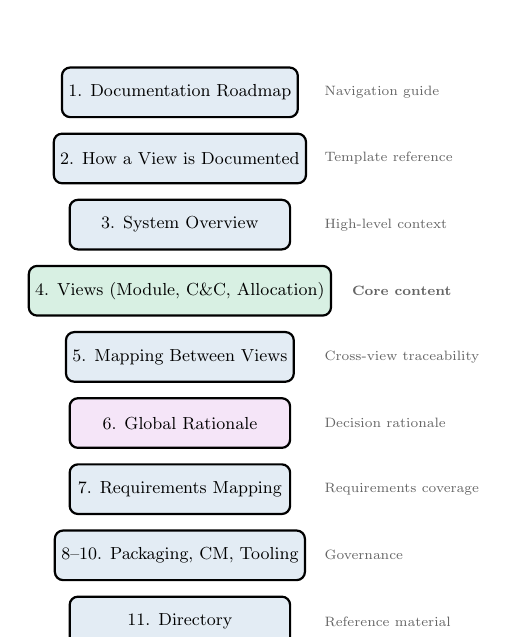
\begin{tikzpicture}[
    scale=0.7,
    transform shape,
    section/.style={draw, thick, fill=modulecolor!15, minimum width=4cm, minimum height=0.9cm, rounded corners=3pt, font=\small},
    arrow/.style={-{Stealth[length=2mm]}, thick, flowcolor}
]
    % Sections
    \node[section] (s1) at (0,6) {1. Documentation Roadmap};
    \node[section] (s2) at (0,4.8) {2. How a View is Documented};
    \node[section] (s3) at (0,3.6) {3. System Overview};
    \node[section, fill=cnccolor!20, minimum width=5cm] (s4) at (0,2.4) {4. Views (Module, C\&C, Allocation)};
    \node[section] (s5) at (0,1.2) {5. Mapping Between Views};
    \node[section, fill=decisioncolor!15] (s6) at (0,0) {6. Global Rationale};
    \node[section] (s7) at (0,-1.2) {7. Requirements Mapping};
    \node[section] (s8) at (0,-2.4) {8--10. Packaging, CM, Tooling};
    \node[section] (s11) at (0,-3.6) {11. Directory};
    
    % Annotations
    \node[right, font=\scriptsize, text=flowcolor] at (2.5,6) {Navigation guide};
    \node[right, font=\scriptsize, text=flowcolor] at (2.5,4.8) {Template reference};
    \node[right, font=\scriptsize, text=flowcolor] at (2.5,3.6) {High-level context};
    \node[right, font=\scriptsize, text=flowcolor] at (3,2.4) {\textbf{Core content}};
    \node[right, font=\scriptsize, text=flowcolor] at (2.5,1.2) {Cross-view traceability};
    \node[right, font=\scriptsize, text=flowcolor] at (2.5,0) {Decision rationale};
    \node[right, font=\scriptsize, text=flowcolor] at (2.5,-1.2) {Requirements coverage};
    \node[right, font=\scriptsize, text=flowcolor] at (2.5,-2.4) {Governance};
    \node[right, font=\scriptsize, text=flowcolor] at (2.5,-3.6) {Reference material};
\end{tikzpicture}
\caption{Document Structure Overview}
\end{figure}

\begin{itemize}
  \item \textbf{Section 1: Documentation Roadmap} --- Orientation to the document structure, stakeholder guidance, and view catalog.
  
  \item \textbf{Section 2: How a View is Documented} --- Standard template used for all architectural views, ensuring consistency and completeness.
  
  \item \textbf{Section 3: System Overview} --- High-level description of \SystemName{} including business context, capabilities, constraints, and stakeholders.
  
  \item \textbf{Section 4: Views} --- The architectural views themselves:
  \begin{itemize}[nosep]
      \item Module views: Decomposition, Uses, Layered, Data Model
      \item Component-and-Connector views: Service-Oriented, Event-Driven
      \item Allocation views: Deployment, Work Assignment
  \end{itemize}
  
  \item \textbf{Section 5: Mapping Between Views} --- How elements correspond across views; rules for navigation and consistency.
  
  \item \textbf{Section 6: Global Rationale} --- Cross-cutting architectural decisions, strategy, and trade-offs affecting multiple views.
  
  \item \textbf{Section 7: Requirements Mapping} --- Traceability between requirements and architectural elements; coverage analysis.
  
  \item \textbf{Section 8: Packaging and Collaboration} --- How documentation is packaged, published online, and maintained collaboratively.
  
  \item \textbf{Section 9: Configuration Management} --- Versioning strategy, release process, and alignment with code releases.
  
  \item \textbf{Section 10: Presentation and Tooling} --- Style guide, notation standards, and supporting tools.
  
  \item \textbf{Section 11: Directory} --- Glossary, acronyms, and references for quick lookup.
\end{itemize}

\subsection{View Overview}

The following table summarizes all architectural views documented for \SystemName.

\setlength{\extrarowheight}{3pt}
\begin{longtable}{@{}L{3cm} L{2.5cm} L{4cm} L{3.5cm}@{}}
\caption{Architectural Views Catalog} \\
\toprule
\textbf{View Name} & \textbf{Style} & \textbf{Primary Concerns} & \textbf{Stakeholders} \\
\midrule
\endfirsthead
\toprule
\textbf{View Name} & \textbf{Style} & \textbf{Primary Concerns} & \textbf{Stakeholders} \\
\midrule
\endhead
\bottomrule
\endlastfoot
Decomposition View & Module & Code organization; team ownership; build structure & Developers; Tech Leads; Build Engineers \\
Uses View & Module & Dependencies; impact analysis; build order & Developers; Architects \\
Layered View & Module & Abstraction levels; portability; dependency rules & Architects; Developers \\
Data Model View & Module & Persistent data structures; data ownership & Data Engineers; DBAs; Developers \\
Service View & C\&C (SOA) & Runtime services; APIs; synchronous communication & Developers; Operations; Integrators \\
Event-Driven View & C\&C (Pub-Sub) & Asynchronous communication; event flows & Developers; Operations \\
Deployment View & Allocation & Infrastructure mapping; scaling; availability & Operations; SREs; Security \\
Work Assignment & Allocation & Team responsibilities; development coordination & Management; Tech Leads \\
\end{longtable}

\subsection{Stakeholders and How They Use the Documentation}

Different stakeholders have different information needs. This table guides each role to the most relevant sections.

\begin{longtable}{@{}L{2.8cm} L{4.5cm} L{5.5cm}@{}}
\caption{Stakeholder Navigation Guide} \\
\toprule
\textbf{Stakeholder} & \textbf{Key Concerns} & \textbf{Recommended Sections} \\
\midrule
\endfirsthead
\toprule
\textbf{Stakeholder} & \textbf{Key Concerns} & \textbf{Recommended Sections} \\
\midrule
\endhead
\bottomrule
\endlastfoot
Executive / Sponsor & Business alignment; risk; investment decisions & System Overview; Global Rationale; Requirements Mapping \\
Product Manager & Feature mapping; capability coverage & System Overview; Requirements Mapping; Service View \\
Software Developer & Component responsibilities; interfaces; dependencies & Decomposition View; Uses View; Service View; Element Catalogs \\
Tech Lead & Team boundaries; integration points; technical decisions & All views; Global Rationale; Work Assignment View \\
Architect & Patterns; trade-offs; quality attribute support & All sections; emphasis on Rationale and Mappings \\
QA Engineer & Testability; component boundaries; scenarios & Service View; Behavior descriptions; Requirements Mapping \\
Operations / SRE & Deployment; monitoring; failure modes & Deployment View; Service View; Event-Driven View \\
Security Engineer & Security mechanisms; trust boundaries; data flows & Layered View; Service View; Deployment View; Global Rationale \\
DBA / Data Engineer & Data models; storage; data flows & Data Model View; Event-Driven View \\
New Team Member & System understanding; orientation & Documentation Roadmap; System Overview; then specific views \\
External Integrator & APIs; integration patterns; protocols & Service View; Context diagrams; Interface documentation \\
\end{longtable}

\begin{bestpractice}
\textbf{Reading Path for New Team Members:}
\begin{enumerate}[nosep]
    \item Start with Section 3 (System Overview) for business context
    \item Read the Decomposition View to understand code structure
    \item Study the Service View to understand runtime behavior
    \item Review Global Rationale to understand key decisions
    \item Consult specific views as needed for assigned work
\end{enumerate}
\end{bestpractice}

\newpage

% ======================================================================
\section{How a View is Documented}
% ======================================================================

This section defines the standard template used for documenting each architectural view. Consistent structure enables efficient navigation and ensures completeness.

\subsection{Standard View Template}

Every architectural view follows this six-part structure:

\begin{figure}[H]
\centering
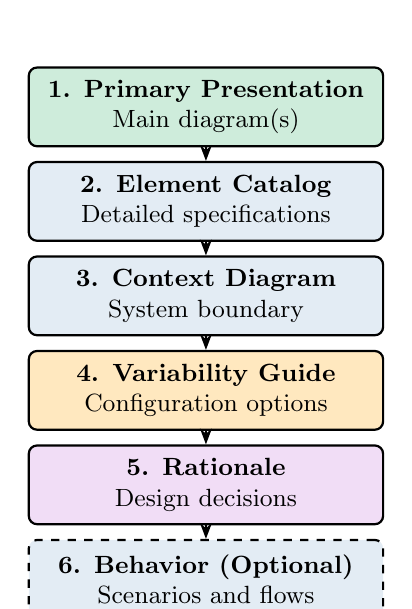
\begin{tikzpicture}[
    scale=0.8,
    part/.style={draw, thick, fill=modulecolor!15, minimum width=4.5cm, minimum height=1cm, rounded corners=3pt, font=\small, align=center},
    arrow/.style={-{Stealth[length=2mm]}, thick}
]
    \node[part, fill=cnccolor!25] (p1) at (0,5) {\textbf{1. Primary Presentation}\\Main diagram(s)};
    \node[part] (p2) at (0,3.5) {\textbf{2. Element Catalog}\\Detailed specifications};
    \node[part] (p3) at (0,2) {\textbf{3. Context Diagram}\\System boundary};
    \node[part, fill=alloccolor!25] (p4) at (0,0.5) {\textbf{4. Variability Guide}\\Configuration options};
    \node[part, fill=decisioncolor!20] (p5) at (0,-1) {\textbf{5. Rationale}\\Design decisions};
    \node[part, dashed] (p6) at (0,-2.5) {\textbf{6. Behavior (Optional)}\\Scenarios and flows};
    
    \draw[arrow] (p1) -- (p2);
    \draw[arrow] (p2) -- (p3);
    \draw[arrow] (p3) -- (p4);
    \draw[arrow] (p4) -- (p5);
    \draw[arrow] (p5) -- (p6);
\end{tikzpicture}
\caption{Standard View Template Structure}
\end{figure}

\begin{enumerate}
  \item \textbf{Primary Presentation} --- The main graphical or textual representation of the view. This is typically one or more diagrams showing the key elements and their relationships, accompanied by a notation key.
  
  \item \textbf{Element Catalog} --- Detailed documentation of each element and relation shown in the primary presentation. Includes element properties, interfaces, behaviors, and constraints.
  
  \item \textbf{Context Diagram} --- Shows the system or subsystem as a black box, depicting its boundary and interactions with external entities.
  
  \item \textbf{Variability Guide} --- Documents variation points: what can be configured, extended, or substituted, along with constraints on valid configurations.
  
  \item \textbf{Rationale} --- Explains why the design is the way it is, including decisions made, alternatives considered, and impact on quality attributes.
  
  \item \textbf{Behavior of the Configuration} (Optional) --- When needed, describes the behavior of the whole configuration rather than individual elements, typically through scenarios or sequence diagrams.
\end{enumerate}

\begin{warning}
Avoid silently omitting sections. If a section does not apply to a particular view, explicitly state ``Not applicable'' or ``None'' with a brief explanation.
\end{warning}

\subsection{View Template Details}

\begin{template}
\textbf{Complete View Documentation Template}

\vspace{0.3cm}
\textbf{View Metadata}
\begin{itemize}[nosep]
    \item \textbf{View Name:} Descriptive name (e.g., ``Service-Oriented View'')
    \item \textbf{View Style:} Category and specific style (e.g., ``C\&C / Service-Oriented Architecture'')
    \item \textbf{Scope:} What portion of the system this view covers
    \item \textbf{Primary Stakeholders:} Roles this view primarily serves
    \item \textbf{Status:} Draft / Review / Approved
    \item \textbf{Last Updated:} Date of last modification
\end{itemize}

\vspace{0.3cm}
\textbf{1. Primary Presentation}
\begin{itemize}[nosep]
    \item Main diagram(s) or textual representation
    \item Notation key explaining all symbols, shapes, colors, and line styles
    \item Brief highlights summarizing what the diagram shows
    \item Multiple diagrams permitted when single diagram would be overcrowded
\end{itemize}

\vspace{0.3cm}
\textbf{2. Element Catalog}
\begin{itemize}[nosep]
    \item \textbf{2.1 Elements and Properties:} For each element type and instance
    \item \textbf{2.2 Relations and Properties:} For each relation type
    \item \textbf{2.3 Element Interfaces:} APIs, contracts, protocols
    \item \textbf{2.4 Element Behavior:} State machines, invariants, constraints
\end{itemize}

\vspace{0.3cm}
\textbf{3. Context Diagram}
\begin{itemize}[nosep]
    \item System/subsystem shown as black box
    \item External actors, systems, and interfaces
    \item Brief narrative explaining key interactions
\end{itemize}

\vspace{0.3cm}
\textbf{4. Variability Guide}
\begin{itemize}[nosep]
    \item Variation points (configuration, plugins, alternatives)
    \item Binding times (compile, deploy, runtime)
    \item Constraints on valid combinations
    \item Instantiation instructions for known variants
\end{itemize}

\vspace{0.3cm}
\textbf{5. Rationale}
\begin{itemize}[nosep]
    \item Key design decisions specific to this view
    \item Alternatives considered and reasons for rejection
    \item Impact on quality attributes
    \item References to ADRs where applicable
\end{itemize}

\vspace{0.3cm}
\textbf{6. Behavior of the Configuration} (when applicable)
\begin{itemize}[nosep]
    \item Key scenarios showing element interactions
    \item Sequence diagrams or collaboration diagrams
    \item Timing constraints or ordering requirements
\end{itemize}
\end{template}

\subsection{Notation Standards}

All views in this document follow these notation conventions:

\begin{longtable}{@{}L{3cm} L{3cm} L{6.5cm}@{}}
\caption{Standard Notation Elements} \\
\toprule
\textbf{Element} & \textbf{Symbol} & \textbf{Usage} \\
\midrule
\endfirsthead
\toprule
\textbf{Element} & \textbf{Symbol} & \textbf{Usage} \\
\midrule
\endhead
\bottomrule
\endlastfoot
Module & Rectangle & Code unit (package, namespace, library) \\
Component & Rectangle with ports & Runtime unit (service, process) \\
Connector & Line with labels & Communication mechanism \\
External System & Dashed rectangle & System outside scope \\
Data Store & Cylinder & Database, file system, cache \\
Actor & Stick figure & Human user or external system \\
Boundary & Dashed border & System or subsystem boundary \\
Layer & Horizontal band & Abstraction level \\
Node & 3D box & Infrastructure element \\
Synchronous call & Solid arrow & Request-response communication \\
Asynchronous message & Dashed arrow & Fire-and-forget or event \\
Data flow & Arrow with label & Data movement direction \\
Dependency & Dashed arrow & ``Uses'' or ``depends on'' \\
Containment & Nesting & Parent-child relationship \\
\end{longtable}

\newpage

% ======================================================================
\section{System Overview}
% ======================================================================

This section provides a high-level understanding of \SystemName{} without committing to any particular view. It establishes shared context for all subsequent architectural descriptions.

\subsection{Problem Statement}

\SystemName{} addresses the need for a modern, scalable e-commerce platform that supports both B2C (business-to-consumer) and B2B (business-to-business) commerce. The platform replaces a legacy monolithic system that has reached its scalability limits and cannot support the business growth targets of 10x transaction volume over five years.

\textbf{Key Business Drivers:}
\begin{itemize}
    \item \textbf{Scalability:} Handle Black Friday traffic peaks of 100,000 concurrent users
    \item \textbf{Global Expansion:} Support multi-region deployment and multi-currency transactions
    \item \textbf{Time-to-Market:} Enable independent deployment of features by autonomous teams
    \item \textbf{Partner Integration:} Provide robust APIs for marketplace sellers and B2B customers
    \item \textbf{Operational Excellence:} Achieve 99.95\% availability with sub-second response times
\end{itemize}

\subsection{System Capabilities}

\SystemName{} provides the following major capabilities:

\begin{longtable}{@{}L{3.5cm} L{9cm}@{}}
\caption{System Capabilities} \\
\toprule
\textbf{Capability} & \textbf{Description} \\
\midrule
\endfirsthead
\toprule
\textbf{Capability} & \textbf{Description} \\
\midrule
\endhead
\bottomrule
\endlastfoot
Product Catalog & Browse, search, and filter products with faceted navigation; support for configurable and bundled products \\
Shopping Cart & Persistent cart with real-time inventory checks; saved for later; gift options \\
Checkout & Multi-step checkout with address validation, tax calculation, shipping options, and payment processing \\
Order Management & Order lifecycle from placement through fulfillment; modifications, cancellations, and returns \\
Inventory Management & Real-time stock levels across warehouses; reservations; backorder management \\
User Management & Registration, authentication, profiles, preferences, and address book \\
Payment Processing & Multiple payment methods; PCI-compliant processing; refunds and disputes \\
Search & Full-text search with relevance ranking, filters, and personalization \\
Notifications & Transactional emails, SMS, and push notifications for order updates \\
Analytics & Business intelligence, funnel analysis, and recommendation engine data \\
Administration & Back-office tools for catalog, inventory, orders, and customer service \\
\end{longtable}

\subsection{Users and External Stakeholders}

\begin{figure}[H]
\centering
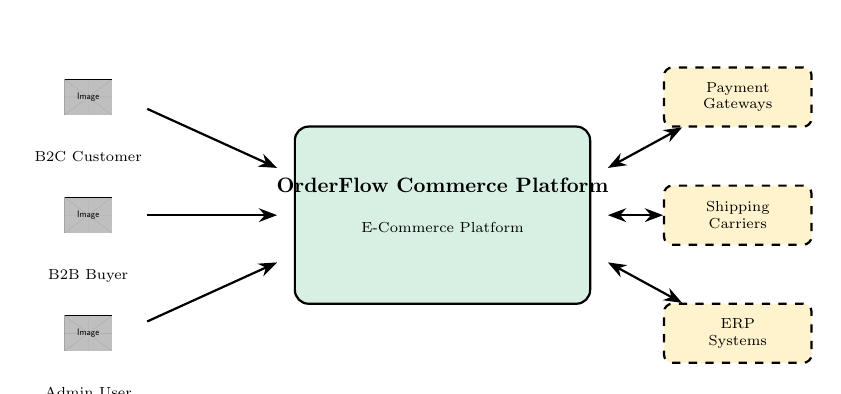
\begin{tikzpicture}[
    scale=0.75,
    transform shape,
    actor/.style={font=\small},
    system/.style={draw, thick, fill=cnccolor!20, minimum width=5cm, minimum height=3cm, rounded corners=5pt},
    external/.style={draw, thick, dashed, fill=externalcolor!20, minimum width=2.5cm, minimum height=1cm, rounded corners=3pt, font=\scriptsize, align=center}
]
    % Central system
    \node[system] (sys) at (0,0) {};
    \node[font=\bfseries] at (0,0.5) {\SystemName};
    \node[font=\scriptsize] at (0,-0.2) {E-Commerce Platform};
    
    % Users (left side)
    \node[actor] at (-6,2) {\includegraphics[width=0.8cm]{example-image}};
    \node[font=\scriptsize, below] at (-6,1.2) {B2C Customer};
    \draw[-{Stealth}, thick] (-5,1.8) -- (-2.8,0.8);
    
    \node[actor] at (-6,0) {\includegraphics[width=0.8cm]{example-image}};
    \node[font=\scriptsize, below] at (-6,-0.8) {B2B Buyer};
    \draw[-{Stealth}, thick] (-5,0) -- (-2.8,0);
    
    \node[actor] at (-6,-2) {\includegraphics[width=0.8cm]{example-image}};
    \node[font=\scriptsize, below] at (-6,-2.8) {Admin User};
    \draw[-{Stealth}, thick] (-5,-1.8) -- (-2.8,-0.8);
    
    % External systems (right side)
    \node[external] (pay) at (5,2) {Payment\\Gateways};
    \draw[{Stealth}-{Stealth}, thick] (2.8,0.8) -- (pay);
    
    \node[external] (ship) at (5,0) {Shipping\\Carriers};
    \draw[{Stealth}-{Stealth}, thick] (2.8,0) -- (ship);
    
    \node[external] (erp) at (5,-2) {ERP\\Systems};
    \draw[{Stealth}-{Stealth}, thick] (2.8,-0.8) -- (erp);
\end{tikzpicture}
\caption{System Context Overview}
\end{figure}

\textbf{User Types:}
\begin{itemize}
    \item \textbf{B2C Customers:} Individual consumers browsing and purchasing products via web and mobile
    \item \textbf{B2B Buyers:} Business purchasers with contract pricing, bulk ordering, and approval workflows
    \item \textbf{Marketplace Sellers:} Third-party merchants listing and fulfilling products
    \item \textbf{Customer Service:} Support agents handling inquiries, orders, and returns
    \item \textbf{Merchandisers:} Business users managing catalog, pricing, and promotions
    \item \textbf{Operations:} Warehouse staff managing inventory and fulfillment
    \item \textbf{Administrators:} IT staff managing system configuration and access
\end{itemize}

\textbf{External Systems:}
\begin{itemize}
    \item Payment gateways (Stripe, PayPal, Adyen)
    \item Shipping carriers (FedEx, UPS, DHL)
    \item Tax calculation services (Avalara)
    \item ERP and financial systems (SAP, NetSuite)
    \item Marketing automation (Salesforce, HubSpot)
    \item Analytics platforms (Google Analytics, Segment)
\end{itemize}

\subsection{Key Constraints and Context}

\begin{longtable}{@{}L{2.5cm} L{3.5cm} L{6.5cm}@{}}
\caption{Architectural Constraints} \\
\toprule
\textbf{Category} & \textbf{Constraint} & \textbf{Impact on Architecture} \\
\midrule
\endfirsthead
\toprule
\textbf{Category} & \textbf{Constraint} & \textbf{Impact on Architecture} \\
\midrule
\endhead
\bottomrule
\endlastfoot
Technical & AWS cloud platform & All infrastructure designed for AWS services \\
Technical & Java/Kotlin primary languages & Service implementation technology stack \\
Technical & PostgreSQL for OLTP & Primary database; influences data model \\
Regulatory & PCI-DSS Level 1 & Payment data isolation; encryption requirements \\
Regulatory & GDPR compliance & Data residency; consent management; right to deletion \\
Organizational & 8 autonomous teams & Microservices aligned with team boundaries \\
Organizational & 2-week sprint cycles & Incremental delivery; feature toggles \\
Schedule & November 2024 launch & MVP scope definition; phased rollout \\
Budget & \$50K/month infrastructure & Cost-optimized architecture; auto-scaling \\
Integration & Legacy system coexistence & Strangler pattern; data synchronization \\
\end{longtable}

\newpage

% ======================================================================
\section{Views}
% ======================================================================

This section contains the architectural views for \SystemName. Each view follows the standard template defined in Section 2.

\subsection{Module Decomposition View}

\begin{viewbox}[Module Decomposition View]

\textbf{View Metadata}
\begin{itemize}[nosep]
    \item \textbf{View Style:} Module / Decomposition
    \item \textbf{Scope:} Entire \SystemName{} platform
    \item \textbf{Primary Stakeholders:} Developers, Tech Leads, Build Engineers
    \item \textbf{Status:} \statusapproved
\end{itemize}

\vspace{0.3cm}
\subsubsection*{1. Primary Presentation}

\begin{figure}[H]
\centering
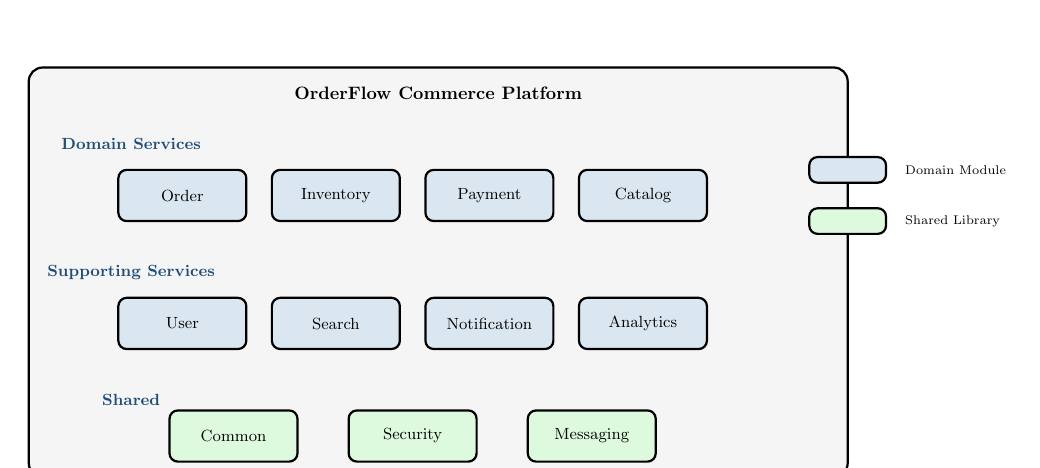
\begin{tikzpicture}[
    scale=0.65,
    transform shape,
    module/.style={draw, thick, fill=modulecolor!20, minimum width=2.5cm, minimum height=1cm, rounded corners=3pt, font=\small},
    shared/.style={draw, thick, fill=datacolor!30, minimum width=2.5cm, minimum height=1cm, rounded corners=3pt, font=\small},
    infra/.style={draw, thick, fill=alloccolor!30, minimum width=2.5cm, minimum height=1cm, rounded corners=3pt, font=\small}
]
    % Top level
    \node[draw, thick, fill=lightgray, minimum width=16cm, minimum height=8cm, rounded corners=5pt] at (0,0) {};
    \node[font=\bfseries] at (0,3.5) {\SystemName};
    
    % Domain Services Layer
    \node[font=\small\bfseries, text=sectionblue] at (-6,2.5) {Domain Services};
    \node[module] (order) at (-5,1.5) {Order};
    \node[module] (inventory) at (-2,1.5) {Inventory};
    \node[module] (payment) at (1,1.5) {Payment};
    \node[module] (catalog) at (4,1.5) {Catalog};
    
    % Supporting Services
    \node[font=\small\bfseries, text=sectionblue] at (-6,0) {Supporting Services};
    \node[module] (user) at (-5,-1) {User};
    \node[module] (search) at (-2,-1) {Search};
    \node[module] (notify) at (1,-1) {Notification};
    \node[module] (analytics) at (4,-1) {Analytics};
    
    % Shared Libraries
    \node[font=\small\bfseries, text=sectionblue] at (-6,-2.5) {Shared};
    \node[shared] (common) at (-4,-3.2) {Common};
    \node[shared] (security) at (-0.5,-3.2) {Security};
    \node[shared] (messaging) at (3,-3.2) {Messaging};
    
    % Legend
    \node[module, minimum width=1.5cm, minimum height=0.5cm] at (8,2) {};
    \node[font=\scriptsize, right] at (9,2) {Domain Module};
    \node[shared, minimum width=1.5cm, minimum height=0.5cm] at (8,1) {};
    \node[font=\scriptsize, right] at (9,1) {Shared Library};
\end{tikzpicture}
\caption{Module Decomposition -- Top Level}
\end{figure}

\textbf{Notation Key:}
\begin{itemize}[nosep]
    \item Blue rectangles: Domain service modules (independently deployable)
    \item Green rectangles: Shared libraries (compile-time dependencies)
    \item Containment: Parent-child module relationship
\end{itemize}

\vspace{0.3cm}
\subsubsection*{2. Element Catalog}

\textbf{2.1 Module Elements}

\begin{longtable}{@{}L{2.2cm} L{4.5cm} L{2cm} L{4cm}@{}}
\toprule
\textbf{Module} & \textbf{Responsibility} & \textbf{Owner} & \textbf{Key Dependencies} \\
\midrule
\endfirsthead
\bottomrule
\endlastfoot
Order & Order lifecycle management from cart to fulfillment & Order Team & Inventory, Payment, User, Common \\
Inventory & Stock levels, reservations, warehouse management & Inventory Team & Common, Messaging \\
Payment & Payment processing, refunds, PCI compliance & Payment Team & Security, Common \\
Catalog & Product information, categories, attributes & Catalog Team & Search, Common \\
User & Authentication, profiles, preferences & Identity Team & Security, Common \\
Search & Full-text search, indexing, relevance & Search Team & Catalog, Common \\
Notification & Email, SMS, push notification delivery & Platform Team & Messaging, Common \\
Analytics & Event collection, metrics, reporting & Data Team & Messaging, Common \\
Common & Shared utilities, DTOs, error handling & Platform Team & None \\
Security & Auth, encryption, audit logging & Security Team & Common \\
Messaging & Event publishing, message contracts & Platform Team & Common \\
\end{longtable}

\vspace{0.3cm}
\subsubsection*{3. Context Diagram}

The module decomposition exists within the broader development ecosystem:

\begin{itemize}[nosep]
    \item \textbf{Build System:} Gradle multi-project build with module dependencies
    \item \textbf{Repository:} Monorepo with module-per-directory structure
    \item \textbf{CI/CD:} Module-level builds triggered by change detection
\end{itemize}

\vspace{0.3cm}
\subsubsection*{4. Variability Guide}

\begin{itemize}[nosep]
    \item \textbf{Feature Modules:} Optional modules (Analytics, Notification) can be excluded from builds
    \item \textbf{Database Providers:} Data access abstracted; PostgreSQL default, MySQL supported
    \item \textbf{Payment Gateways:} Plugin architecture for payment provider adapters
\end{itemize}

\vspace{0.3cm}
\subsubsection*{5. Rationale}

\textbf{Key Decisions:}
\begin{itemize}[nosep]
    \item \textbf{Domain-Driven Decomposition:} Modules align with business domains for team autonomy (ADR-003)
    \item \textbf{Shared Libraries over Services:} Common code as libraries reduces runtime coupling (ADR-007)
    \item \textbf{Monorepo:} Single repository enables atomic changes across modules (ADR-005)
\end{itemize}

\textbf{Quality Attribute Support:}
\begin{itemize}[nosep]
    \item \textbf{Modifiability:} Clear boundaries enable independent module evolution
    \item \textbf{Testability:} Module isolation facilitates unit and integration testing
    \item \textbf{Buildability:} Gradle module dependencies enable parallel builds
\end{itemize}

\end{viewbox}

\subsection{Service-Oriented (C\&C) View}

\begin{viewbox}[Service-Oriented View]

\textbf{View Metadata}
\begin{itemize}[nosep]
    \item \textbf{View Style:} Component-and-Connector / Service-Oriented Architecture
    \item \textbf{Scope:} Runtime services and synchronous communication
    \item \textbf{Primary Stakeholders:} Developers, Operations, Integrators
    \item \textbf{Status:} \statusapproved
\end{itemize}

\vspace{0.3cm}
\subsubsection*{1. Primary Presentation}

\begin{figure}[H]
\centering
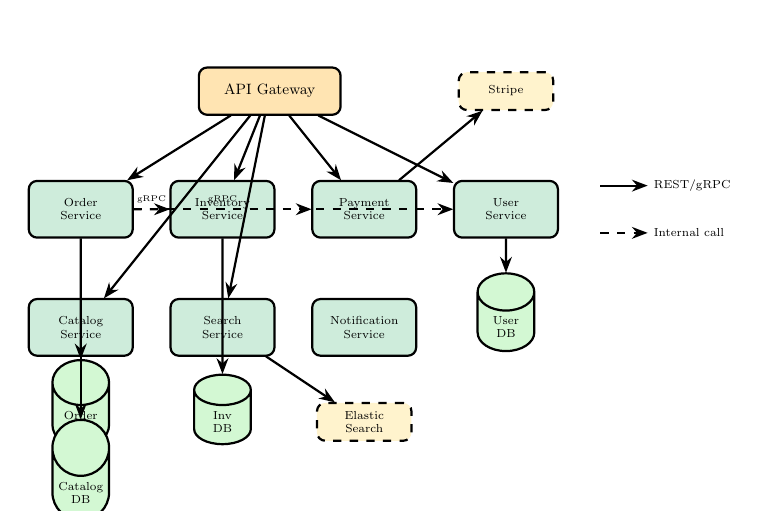
\begin{tikzpicture}[
    scale=0.6,
    transform shape,
    service/.style={draw, thick, fill=cnccolor!25, minimum width=2.2cm, minimum height=1.2cm, rounded corners=3pt, font=\scriptsize, align=center},
    gateway/.style={draw, thick, fill=alloccolor!30, minimum width=3cm, minimum height=1cm, rounded corners=3pt, font=\small, align=center},
    db/.style={draw, thick, fill=datacolor!40, cylinder, shape border rotate=90, minimum width=1.2cm, minimum height=0.8cm, font=\scriptsize, align=center},
    external/.style={draw, thick, dashed, fill=externalcolor!20, minimum width=2cm, minimum height=0.8cm, rounded corners=3pt, font=\scriptsize, align=center},
    arrow/.style={-{Stealth[length=2mm]}, thick}
]
    % API Gateway
    \node[gateway] (gw) at (0,4) {API Gateway};
    
    % Services
    \node[service] (order) at (-4,1.5) {Order\\Service};
    \node[service] (inv) at (-1,1.5) {Inventory\\Service};
    \node[service] (pay) at (2,1.5) {Payment\\Service};
    \node[service] (user) at (5,1.5) {User\\Service};
    
    \node[service] (catalog) at (-4,-1) {Catalog\\Service};
    \node[service] (search) at (-1,-1) {Search\\Service};
    \node[service] (notify) at (2,-1) {Notification\\Service};
    
    % Databases
    \node[db] (orderdb) at (-4,-3) {Order\\DB};
    \node[db] (invdb) at (-1,-3) {Inv\\DB};
    \node[db] (userdb) at (5,-1) {User\\DB};
    \node[db] (catdb) at (-4,-4.5) {Catalog\\DB};
    
    % External
    \node[external] (stripe) at (5,4) {Stripe};
    \node[external] (elastic) at (2,-3) {Elastic\\Search};
    
    % Connections from gateway
    \draw[arrow] (gw) -- (order);
    \draw[arrow] (gw) -- (inv);
    \draw[arrow] (gw) -- (pay);
    \draw[arrow] (gw) -- (user);
    \draw[arrow] (gw) -- (catalog);
    \draw[arrow] (gw) -- (search);
    
    % Service to service
    \draw[arrow, dashed] (order) -- node[above, font=\tiny] {gRPC} (inv);
    \draw[arrow, dashed] (order) -- node[above, font=\tiny] {gRPC} (pay);
    \draw[arrow, dashed] (order) -- (user);
    
    % Service to DB
    \draw[arrow] (order) -- (orderdb);
    \draw[arrow] (inv) -- (invdb);
    \draw[arrow] (user) -- (userdb);
    \draw[arrow] (catalog) -- (catdb);
    \draw[arrow] (search) -- (elastic);
    
    % External
    \draw[arrow] (pay) -- (stripe);
    
    % Legend
    \draw[arrow] (7,2) -- (8,2) node[right, font=\scriptsize] {REST/gRPC};
    \draw[arrow, dashed] (7,1) -- (8,1) node[right, font=\scriptsize] {Internal call};
\end{tikzpicture}
\caption{Service-Oriented View -- Runtime Components}
\end{figure}

\vspace{0.3cm}
\subsubsection*{2. Element Catalog}

\textbf{2.1 Service Components}

\begin{longtable}{@{}L{2.3cm} L{3cm} L{2cm} L{2cm} L{3cm}@{}}
\toprule
\textbf{Service} & \textbf{API Style} & \textbf{Instances} & \textbf{SLA} & \textbf{Data Store} \\
\midrule
\endfirsthead
\bottomrule
\endlastfoot
API Gateway & REST, GraphQL & 3 & 99.99\% & Redis (session) \\
Order Service & REST, gRPC & 5 & 99.95\% & PostgreSQL \\
Inventory Service & gRPC & 3 & 99.95\% & PostgreSQL \\
Payment Service & REST & 3 & 99.99\% & PostgreSQL (encrypted) \\
User Service & REST & 3 & 99.95\% & PostgreSQL \\
Catalog Service & REST & 3 & 99.9\% & PostgreSQL \\
Search Service & REST & 2 & 99.9\% & Elasticsearch \\
Notification Service & REST & 2 & 99.5\% & PostgreSQL \\
\end{longtable}

\textbf{2.3 Service Interfaces}

Each service exposes:
\begin{itemize}[nosep]
    \item REST API documented via OpenAPI 3.0 specification
    \item gRPC interfaces defined in Protocol Buffer files (for internal communication)
    \item Health check endpoint (\texttt{/health}) for orchestrator probes
    \item Metrics endpoint (\texttt{/metrics}) for Prometheus scraping
\end{itemize}

\vspace{0.3cm}
\subsubsection*{5. Rationale}

\textbf{Key Decisions:}
\begin{itemize}[nosep]
    \item \textbf{API Gateway Pattern:} Centralized entry point for cross-cutting concerns (ADR-011)
    \item \textbf{gRPC for Internal:} Binary protocol reduces latency for service-to-service calls (ADR-014)
    \item \textbf{Database per Service:} Data isolation enables independent scaling and evolution (ADR-008)
\end{itemize}

\end{viewbox}

\subsection{Deployment View}

\begin{viewbox}[Deployment View]

\textbf{View Metadata}
\begin{itemize}[nosep]
    \item \textbf{View Style:} Allocation / Deployment
    \item \textbf{Scope:} Production infrastructure
    \item \textbf{Primary Stakeholders:} Operations, SREs, Security
    \item \textbf{Status:} \statusapproved
\end{itemize}

\vspace{0.3cm}
\subsubsection*{1. Primary Presentation}

\begin{figure}[H]
\centering
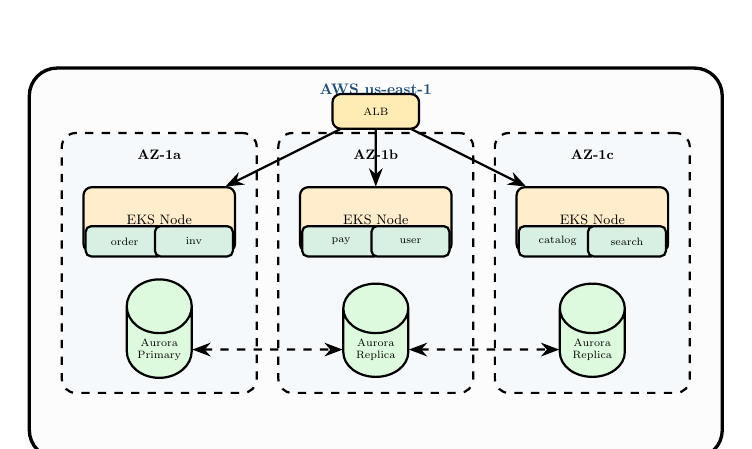
\begin{tikzpicture}[
    scale=0.55,
    transform shape,
    node/.style={draw, thick, fill=alloccolor!20, minimum width=3cm, minimum height=1.5cm, rounded corners=3pt, font=\small, align=center},
    pod/.style={draw, thick, fill=cnccolor!20, minimum width=1.8cm, minimum height=0.7cm, rounded corners=2pt, font=\scriptsize},
    zone/.style={draw, thick, dashed, fill=modulecolor!5, rounded corners=5pt},
    db/.style={draw, thick, fill=datacolor!30, cylinder, shape border rotate=90, minimum width=1.5cm, minimum height=1cm, font=\scriptsize, align=center}
]
    % AWS Cloud boundary
    \node[draw, very thick, fill=lightgray!30, minimum width=16cm, minimum height=9cm, rounded corners=10pt] at (0,0) {};
    \node[font=\bfseries, text=sectionblue] at (0,4) {AWS us-east-1};
    
    % AZ 1
    \node[zone, minimum width=4.5cm, minimum height=6cm] (az1) at (-5,0) {};
    \node[font=\small\bfseries] at (-5,2.5) {AZ-1a};
    \node[node, minimum width=3.5cm] (k8s1) at (-5,1) {EKS Node};
    \node[pod] at (-5.8,0.5) {order};
    \node[pod] at (-4.2,0.5) {inv};
    \node[db] (db1) at (-5,-2) {Aurora\\Primary};
    
    % AZ 2
    \node[zone, minimum width=4.5cm, minimum height=6cm] (az2) at (0,0) {};
    \node[font=\small\bfseries] at (0,2.5) {AZ-1b};
    \node[node, minimum width=3.5cm] (k8s2) at (0,1) {EKS Node};
    \node[pod] at (-0.8,0.5) {pay};
    \node[pod] at (0.8,0.5) {user};
    \node[db] (db2) at (0,-2) {Aurora\\Replica};
    
    % AZ 3
    \node[zone, minimum width=4.5cm, minimum height=6cm] (az3) at (5,0) {};
    \node[font=\small\bfseries] at (5,2.5) {AZ-1c};
    \node[node, minimum width=3.5cm] (k8s3) at (5,1) {EKS Node};
    \node[pod] at (4.2,0.5) {catalog};
    \node[pod] at (5.8,0.5) {search};
    \node[db] (db3) at (5,-2) {Aurora\\Replica};
    
    % Load balancer
    \node[draw, thick, fill=externalcolor!30, minimum width=2cm, minimum height=0.8cm, rounded corners=3pt, font=\scriptsize] (alb) at (0,3.5) {ALB};
    
    % Connections
    \draw[-{Stealth}, thick] (alb) -- (k8s1);
    \draw[-{Stealth}, thick] (alb) -- (k8s2);
    \draw[-{Stealth}, thick] (alb) -- (k8s3);
    
    \draw[{Stealth}-{Stealth}, thick, dashed] (db1) -- (db2);
    \draw[{Stealth}-{Stealth}, thick, dashed] (db2) -- (db3);
\end{tikzpicture}
\caption{Deployment View -- Multi-AZ Production}
\end{figure}

\vspace{0.3cm}
\subsubsection*{2. Element Catalog}

\begin{longtable}{@{}L{2.5cm} L{2.5cm} L{2.5cm} L{5cm}@{}}
\toprule
\textbf{Element} & \textbf{Type} & \textbf{Quantity} & \textbf{Specifications} \\
\midrule
\endfirsthead
\bottomrule
\endlastfoot
EKS Cluster & Kubernetes & 1 & v1.28, 3 AZs, managed control plane \\
Worker Nodes & EC2 & 6-12 & m6i.xlarge, auto-scaling group \\
Aurora PostgreSQL & RDS & 1 cluster & r6g.xlarge, 3 instances, Multi-AZ \\
ElastiCache Redis & Managed & 1 cluster & r6g.large, 3 nodes, cluster mode \\
ALB & Load Balancer & 2 & Internet-facing + internal \\
S3 & Object Storage & 3 buckets & Assets, backups, logs \\
CloudFront & CDN & 1 dist & Global edge locations \\
\end{longtable}

\vspace{0.3cm}
\subsubsection*{5. Rationale}

\textbf{Key Decisions:}
\begin{itemize}[nosep]
    \item \textbf{Multi-AZ Deployment:} Survives single AZ failure; 99.95\% availability target (ADR-015)
    \item \textbf{EKS over ECS:} Kubernetes portability; team expertise; ecosystem (ADR-003)
    \item \textbf{Aurora over RDS PostgreSQL:} Auto-scaling storage; faster failover (ADR-001)
\end{itemize}

\end{viewbox}

\subsection{View Packets}

For large systems, view packets provide focused slices for specific subsystems or stakeholder groups.

\begin{longtable}{@{}L{2.5cm} L{3.5cm} L{4cm} L{3cm}@{}}
\caption{View Packets Registry} \\
\toprule
\textbf{Packet ID} & \textbf{Scope} & \textbf{Contained Views} & \textbf{Stakeholders} \\
\midrule
\endfirsthead
\bottomrule
\endlastfoot
VP-ORDER & Order processing subsystem & Order module decomposition; Order service C\&C; Order data model & Order Team \\
VP-PAYMENT & Payment processing & Payment module; Payment service; PCI deployment & Payment Team; Security \\
VP-SEARCH & Search infrastructure & Search module; Search service; Elasticsearch deployment & Search Team \\
VP-SECURITY & Security architecture & Security module; Auth flows; Security deployment zones & Security Team \\
\end{longtable}

\newpage

% ======================================================================
\section{Mapping Between Views}
% ======================================================================

This section explains how elements in different views correspond, enabling navigation across views and ensuring consistency.

\subsection{Mapping Rules}

\begin{bestpractice}
\textbf{Element Naming Convention:}
\begin{itemize}[nosep]
    \item Same name across views implies same conceptual element
    \item Module ``Order'' maps to service ``Order Service'' maps to deployment ``order-service-pod''
    \item When names differ, explicit mapping is provided in tables below
\end{itemize}
\end{bestpractice}

\subsection{Module to Service Mapping}

\begin{longtable}{@{}L{3.5cm} L{3.5cm} L{2.5cm} L{3cm}@{}}
\caption{Module to Runtime Service Mapping} \\
\toprule
\textbf{Module} & \textbf{Service Component} & \textbf{Relationship} & \textbf{Notes} \\
\midrule
\endfirsthead
\bottomrule
\endlastfoot
Order & Order Service & implements & 1:1 mapping \\
Inventory & Inventory Service & implements & 1:1 mapping \\
Payment & Payment Service & implements & 1:1 mapping \\
Catalog & Catalog Service & implements & 1:1 mapping \\
User & User Service & implements & 1:1 mapping \\
Search & Search Service & implements & 1:1 mapping \\
Notification & Notification Service & implements & 1:1 mapping \\
Analytics & Analytics Service & implements & 1:1 mapping \\
Common & (embedded) & compiled-into & Library, not runtime \\
Security & (embedded) & compiled-into & Library, not runtime \\
Messaging & (embedded) & compiled-into & Library, not runtime \\
\end{longtable}

\subsection{Service to Deployment Mapping}

\begin{longtable}{@{}L{3cm} L{3cm} L{3cm} L{3.5cm}@{}}
\caption{Service to Infrastructure Mapping} \\
\toprule
\textbf{Service} & \textbf{K8s Deployment} & \textbf{Database} & \textbf{Cache} \\
\midrule
\endfirsthead
\bottomrule
\endlastfoot
Order Service & order-deployment & order-db (Aurora) & order-cache (Redis) \\
Inventory Service & inventory-deployment & inventory-db (Aurora) & inventory-cache (Redis) \\
Payment Service & payment-deployment & payment-db (Aurora) & -- \\
User Service & user-deployment & user-db (Aurora) & session-cache (Redis) \\
Catalog Service & catalog-deployment & catalog-db (Aurora) & catalog-cache (Redis) \\
Search Service & search-deployment & -- & -- \\
API Gateway & gateway-deployment & -- & rate-limit-cache (Redis) \\
\end{longtable}

\newpage

% ======================================================================
\section{Global Rationale}
% ======================================================================

This section captures cross-cutting architectural decisions and system-wide trade-offs that affect multiple views.

\subsection{Architecture Strategy}

\SystemName{} follows a \textbf{microservices architecture} with \textbf{event-driven integration}, designed to support:
\begin{itemize}
    \item Independent deployment by autonomous teams
    \item Horizontal scaling of individual services
    \item Technology diversity where beneficial
    \item Resilience through isolation and graceful degradation
\end{itemize}

\textbf{Architectural Styles Applied:}
\begin{itemize}
    \item \textbf{Microservices:} Domain-driven service decomposition
    \item \textbf{Event-Driven:} Asynchronous communication via Kafka
    \item \textbf{API Gateway:} Centralized entry point and cross-cutting concerns
    \item \textbf{CQRS:} Separate read models for search and reporting
    \item \textbf{Database per Service:} Data isolation and autonomy
\end{itemize}

\subsection{Key Cross-Cutting Decisions}

\begin{decisionbox}[ADR-001: Aurora PostgreSQL for Primary Storage]
\textbf{Context:} Need reliable, scalable relational storage for transactional data.

\textbf{Decision:} Use Amazon Aurora PostgreSQL for all primary data stores.

\textbf{Consequences:}
\begin{itemize}[nosep]
    \item (+) Auto-scaling storage; fast failover; managed backups
    \item (+) PostgreSQL compatibility; team expertise
    \item (-) AWS lock-in for database tier
    \item (-) Higher cost than self-managed PostgreSQL
\end{itemize}
\end{decisionbox}

\begin{decisionbox}[ADR-002: Event-Driven Architecture with Kafka]
\textbf{Context:} Services need to communicate without tight coupling; audit trail required.

\textbf{Decision:} Use Apache Kafka (Amazon MSK) for asynchronous event-driven communication.

\textbf{Consequences:}
\begin{itemize}[nosep]
    \item (+) Loose coupling between services
    \item (+) Event replay for recovery and debugging
    \item (+) Natural audit log of all state changes
    \item (-) Eventual consistency complexity
    \item (-) Operational overhead for Kafka cluster
\end{itemize}
\end{decisionbox}

\begin{decisionbox}[ADR-003: Kubernetes (EKS) for Container Orchestration]
\textbf{Context:} Need container orchestration for microservices deployment.

\textbf{Decision:} Use Amazon EKS for Kubernetes-based container orchestration.

\textbf{Consequences:}
\begin{itemize}[nosep]
    \item (+) Industry-standard orchestration; rich ecosystem
    \item (+) Portability to other clouds if needed
    \item (+) Strong team Kubernetes expertise
    \item (-) Complexity compared to simpler options (ECS)
    \item (-) Steeper learning curve for operations
\end{itemize}
\end{decisionbox}

\subsection{Impact on Quality Attributes}

\begin{longtable}{@{}L{2.5cm} L{3cm} L{7cm}@{}}
\caption{Architecture Support for Quality Attributes} \\
\toprule
\textbf{Quality} & \textbf{Target} & \textbf{Architectural Support} \\
\midrule
\endfirsthead
\bottomrule
\endlastfoot
Performance & $<$500ms p95 & CDN caching; Redis caching; gRPC internal calls; read replicas \\
Availability & 99.95\% & Multi-AZ deployment; auto-scaling; circuit breakers; health checks \\
Scalability & 100K concurrent & Horizontal pod scaling; database read replicas; Kafka partitioning \\
Security & PCI-DSS L1 & Network isolation; encryption at rest/transit; secret management \\
Modifiability & 1-day deploy & Microservices isolation; feature flags; backward-compatible APIs \\
Testability & 80\% coverage & Service isolation; contract testing; test containers \\
\end{longtable}

\subsection{Open Questions}

\begin{longtable}{@{}L{1cm} L{4.5cm} L{4cm} L{3cm}@{}}
\caption{Open Architectural Questions} \\
\toprule
\textbf{ID} & \textbf{Question} & \textbf{Impact} & \textbf{Target Date} \\
\midrule
\endfirsthead
\bottomrule
\endlastfoot
OQ-1 & Multi-region deployment strategy? & Affects all views; latency; data residency & Q4 2024 \\
OQ-2 & GraphQL federation approach? & Gateway architecture; team coordination & Q3 2024 \\
OQ-3 & Machine learning platform integration? & New services; data pipelines & Q1 2025 \\
\end{longtable}

\newpage

% ======================================================================
\section{Requirements Mapping}
% ======================================================================

This section demonstrates traceability between requirements and architectural elements.

\subsection{Mapping Strategy}

Requirements are mapped to architecture using a centralized traceability matrix maintained in this document and synchronized with the requirements management tool (Jira). Each requirement is traced to:
\begin{itemize}
    \item Architectural views that address it
    \item Specific elements responsible for satisfying it
    \item Validation approach (how satisfaction is verified)
\end{itemize}

\subsection{Requirements Traceability Matrix}

\begin{longtable}{@{}L{1.5cm} L{3.5cm} L{1.5cm} L{4cm} L{2.5cm}@{}}
\caption{Requirements Traceability Matrix} \\
\toprule
\textbf{Req ID} & \textbf{Summary} & \textbf{Type} & \textbf{Addressed By} & \textbf{Validation} \\
\midrule
\endfirsthead
\toprule
\textbf{Req ID} & \textbf{Summary} & \textbf{Type} & \textbf{Addressed By} & \textbf{Validation} \\
\midrule
\endhead
\bottomrule
\endlastfoot
FR-001 & User registration and login & Func & User Service; Security module & Integration test \\
FR-002 & Product search with filters & Func & Search Service; Elasticsearch & E2E test \\
FR-003 & Shopping cart management & Func & Order Service; Redis cache & Integration test \\
FR-004 & Order placement & Func & Order Service; Payment Service & E2E test \\
FR-005 & Payment processing & Func & Payment Service; Stripe integration & Contract test \\
QA-001 & 99.95\% availability & Quality & Multi-AZ deployment; auto-scaling & SLA monitoring \\
QA-002 & $<$500ms response (p95) & Quality & CDN; caching; gRPC & Load testing \\
QA-003 & 100K concurrent users & Quality & Horizontal scaling; Kubernetes & Load testing \\
QA-004 & PCI-DSS compliance & Quality & Payment isolation; encryption & Audit \\
CON-001 & AWS cloud platform & Constraint & All deployment elements & Architecture review \\
CON-002 & GDPR data residency & Constraint & EU region deployment & Compliance audit \\
\end{longtable}

\newpage

% ======================================================================
\section{Packaging, Online Documentation, and Collaboration}
% ======================================================================

\subsection{Packaging Scheme}

Architecture documentation is packaged for different audiences:

\begin{longtable}{@{}L{3.5cm} L{4cm} L{5cm}@{}}
\caption{Documentation Packages} \\
\toprule
\textbf{Package} & \textbf{Contents} & \textbf{Audience} \\
\midrule
\endfirsthead
\bottomrule
\endlastfoot
Full Architecture Doc & Complete document (this) & Architects; Tech Leads \\
Executive Summary & System Overview; Key Decisions (5 pages) & Executives; Sponsors \\
Developer Guide & Decomposition; Service views; Interfaces & Developers \\
Operations Guide & Deployment view; Runbooks & SREs; Operations \\
Security Package & Security architecture; Threat model & Security Team; Auditors \\
Onboarding Package & Overview; Key views; Glossary & New team members \\
\end{longtable}

\subsection{Online Documentation}

\begin{itemize}
    \item \textbf{Wiki Root:} \texttt{wiki.company.com/architecture/orderflow}
    \item \textbf{One Page per View:} Each view has dedicated wiki page with embedded diagrams
    \item \textbf{Diagram Source:} Stored in Git alongside documentation; exported to wiki
    \item \textbf{Search:} Full-text search enabled across all architecture pages
    \item \textbf{Notifications:} Subscribers notified of significant updates
\end{itemize}

\newpage

% ======================================================================
\section{Configuration Management and Release Strategy}
% ======================================================================

\subsection{Configuration Management}

\begin{itemize}
    \item \textbf{Repository:} \texttt{github.com/company/orderflow-architecture}
    \item \textbf{Branch Strategy:} \texttt{main} for approved content; feature branches for changes
    \item \textbf{Tagging:} Semantic versioning aligned with major system releases
    \item \textbf{Code Alignment:} Architecture doc version noted in system release notes
\end{itemize}

\subsection{Release Strategy}

\begin{itemize}
    \item \textbf{Major Releases:} Aligned with system major versions; full review cycle
    \item \textbf{Minor Updates:} Monthly for accumulated changes; Tech Lead approval
    \item \textbf{Patches:} As needed for corrections; peer review sufficient
    \item \textbf{Communication:} Release notes to \texttt{architecture-announce@company.com}
\end{itemize}

\newpage

% ======================================================================
\section{Presentation and Tooling}
% ======================================================================

\subsection{Presentation and Style Guide}

\begin{itemize}
    \item \textbf{Document Format:} LaTeX source; PDF output; wiki mirror
    \item \textbf{Diagrams:} TikZ for embedded; draw.io/Lucidchart for complex diagrams
    \item \textbf{Fonts:} Latin Modern (LaTeX default); consistent sizing
    \item \textbf{Colors:} Consistent palette defined in document preamble
    \item \textbf{Terminology:} As defined in Glossary; consistent throughout
\end{itemize}

\subsection{Tooling}

\begin{longtable}{@{}L{3cm} L{3.5cm} L{6cm}@{}}
\caption{Architecture Documentation Tools} \\
\toprule
\textbf{Purpose} & \textbf{Tool} & \textbf{Usage} \\
\midrule
\endfirsthead
\bottomrule
\endlastfoot
Document authoring & LaTeX, VS Code & Primary document creation \\
Diagrams & TikZ, draw.io, Lucidchart & Architecture diagrams \\
Version control & Git, GitHub & Source management; reviews \\
Wiki & Confluence & Online documentation \\
Modeling & Structurizr & C4 model diagrams \\
API docs & OpenAPI, Swagger UI & Interface documentation \\
ADRs & Markdown, adr-tools & Decision records \\
\end{longtable}

\newpage

% ======================================================================
\section{Directory}
% ======================================================================

\subsection{Glossary}

\begin{longtable}{@{}L{3.5cm} L{9cm}@{}}
\caption{Glossary of Terms} \\
\toprule
\textbf{Term} & \textbf{Definition} \\
\midrule
\endfirsthead
\bottomrule
\endlastfoot
Architecture View & A representation of a system from the perspective of a related set of concerns \\
Component & A runtime entity that provides or consumes services through interfaces \\
Connector & A runtime pathway for interaction between components \\
Element & A fundamental piece of architecture (module, component, or node) \\
Module & A code unit that implements a coherent set of responsibilities \\
Primary Presentation & The main graphical or textual representation of a view \\
Quality Attribute & A measurable property of a system (performance, availability, etc.) \\
Stakeholder & An individual or organization with interests in the system \\
View Packet & A focused subset of views for a specific subsystem or audience \\
Viewpoint & A specification of conventions for constructing and using a view \\
\end{longtable}

\subsection{Acronyms}

\begin{longtable}{@{}L{2.5cm} L{10cm}@{}}
\caption{Acronyms} \\
\toprule
\textbf{Acronym} & \textbf{Meaning} \\
\midrule
\endfirsthead
\bottomrule
\endlastfoot
ADR & Architecture Decision Record \\
ALB & Application Load Balancer \\
API & Application Programming Interface \\
C\&C & Component-and-Connector \\
CDN & Content Delivery Network \\
CQRS & Command Query Responsibility Segregation \\
EKS & Elastic Kubernetes Service \\
gRPC & Google Remote Procedure Call \\
MSK & Managed Streaming for Apache Kafka \\
PCI-DSS & Payment Card Industry Data Security Standard \\
RDS & Relational Database Service \\
SLA & Service Level Agreement \\
SRE & Site Reliability Engineering \\
\end{longtable}

\subsection{References}

\begin{enumerate}
    \item Clements, P., et al. (2010). \textit{Documenting Software Architectures: Views and Beyond} (2nd ed.). Addison-Wesley.
    
    \item Bass, L., Clements, P., \& Kazman, R. (2021). \textit{Software Architecture in Practice} (4th ed.). Addison-Wesley.
    
    \item ISO/IEC/IEEE 42010:2011. \textit{Systems and software engineering --- Architecture description}.
    
    \item Keeling, M. (2017). \textit{Design It! From Programmer to Software Architect}. Pragmatic Bookshelf.
    
    \item Brown, S. (2018). \textit{The C4 Model for Visualising Software Architecture}. Leanpub.
    
    \item Nygard, M. (2007). \textit{Release It! Design and Deploy Production-Ready Software}. Pragmatic Bookshelf.
    
    \item Newman, S. (2021). \textit{Building Microservices} (2nd ed.). O'Reilly Media.
    
    \item Fowler, M. (2002). \textit{Patterns of Enterprise Application Architecture}. Addison-Wesley.
\end{enumerate}

\end{document}